\chapter{Graph}

\section{Overview and Motivation} 
\label{sec:s1}
   The graph is a pervasive structure which appears in many Computer Science problems. A graph (G = (V,E)) in its basic form is simply a set of vertices (V) and edges (E; storing connectivity information between vertices in V). Later in the next section, we will explore many important graph problems and algorithms. To prepare ourselves, we will discuss three basic ways (there are a few other rare structures) to represent a graph G with V vertices and E edges in this subsection20. Many real-life problems can be classified as graph problems. Some have efficient solutions. Some do not have them yet.   
   \\
   
   In this relatively chapter, we discuss graph problems that commonly appear in real life, the algorithms to solve them, and the practical implementations of these algorithms. We cover topics ranging from basic graph traversals, minimum spanning trees, single-source/all-pairs shortest paths, and discuss graphs with special properties. In computer science, a graph is an abstract data type that is meant to implement the undirected graph and directed graph concepts from mathematics; specifically, the field of graph theory. A graph data structure consists of a finite (and possibly mutable) set of vertices (also called nodes or points), together with a set of unordered pairs of these vertices for an undirected graph or a set of ordered pairs for a directed graph. These pairs are known as edges (also called links or lines), and for a directed graph are also known as arrows. The vertices may be part of the graph structure, or may be external entities represented by integer indices or references. A graph data structure may also associate to each edge some edge value, such as a symbolic label or a numeric attribute (cost, capacity, length, etc.)in figure \ref{fig:GraphRepresentation}.
\newpage

\\
\newline
\textbf{{\Large{So, we can assume the Backtracking function as following:}}}


\begin{lstlisting}{c++}
        void backtrack(state) {
        if (hit end state or invalid state) // we need terminating or
            return; // pruning condition to avoid cycling and to speed up search
        for each neighbor of this state // try all permutation
             backtrack(neighbor);
        }
\end{lstlisting}
\\
\newline
\begin{figure}[h]
    % \centering
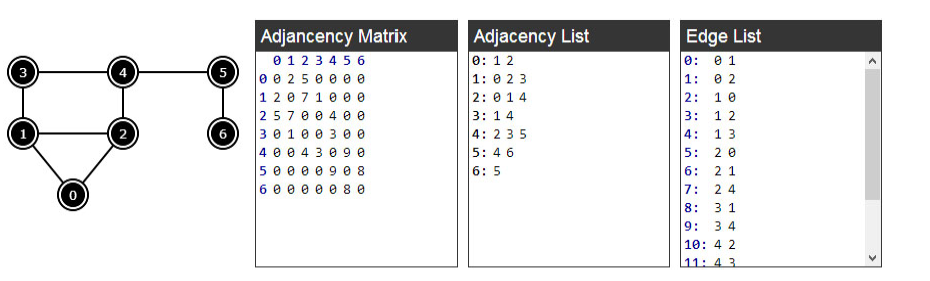
\includegraphics[width=15cm, height=5cm]{GraphRepresentation.png}
 \caption{Graph Data Structure Visualization}
    \label{fig:GraphRepresentation}
\end{figure}


\subsection{Applications}
Graph Applications appear in many problems. Like:
\begin{itemize}
\item Graph Traversing: 

Using DFS (Depth first search) and BFS (Breadth first search).
\item Finding Connected Components (Undirected Graphs) and Flood Fill -Labeling/Coloring the Connected Components-.
\item Topological Sort (Dircyed Acyclic Graph). Using DFS + stack or vector. Or Khan's Algorithm.
\item Graph Edges Property check via DFS Spanning Tree.
\item Finding Articulation Points and Bridges (Undirected Graph). \item Finding Strongly Connected Components (Directed Graph). Using Tarjan's Algorithm.
\item Finding Minimum Spanning Tree. Using Kruskal’s Algorithm and Prim’s Algorithm.
\item Finding Shortest Path Algorithms included Single-Source Shortest Paths:

SSSP on Unweighted Graph, SSSP on Weighted Graph and SSSP on Graph with Negative Weight Cycle and All-Pairs Shortest Paths -Explanation of Floyd Warshall’s DP Solution. 
\item Finding maximum flow using Edmonds Karp’s algorithm and Hopcroft Karp’s algorithm.
\end{itemize}

\newpage
\section{Graph Traversel}
This section discusses two fundamental graph algorithms: depth-first search and breadth-first search. Both algorithms are given a starting node in the graph, and they visit all nodes that can be reached from the starting node. The difference in the algorithms is the order in which they visit the nodes.
\subsection{Depth First Search (DFS) }\label{subsection:DFS}
Depth First Search is one of the main graph algorithms. Depth First Search finds the lexicographical first path in the graph from a source vertex u to each vertex. Depth First Search will also find the shortest paths in a tree (because there only exists one simple path), but on general graphs this is not the case. The algorithm works in O(m+n) time where n is the number of vertices and m is the number of edges.

\subsubsection{Example}\ref{subsection:DFS}
Let us consider how depth-first search processes the following graph:

\begin{figure}[h]
    \centering
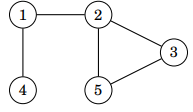
\includegraphics[width=5cm, height=3cm]{graph-example.png}
 \caption{Sample Graph}
    \label{fig:graph-example}
\end{figure}

We may begin the search at any node of the graph. So, let's start traversing at node 1. After that, searching will traversing node 2:

\begin{figure}[h]
    \centering
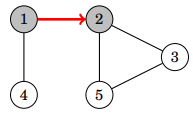
\includegraphics[width=5cm, height=3cm]{graph-example-traverse-1.png}
 \caption{step 1: Sample Graph After Traversing}
    \label{fig:graph-example-traverse-1}
\end{figure}

\newpage

After this, nodes 3 and 5 will be visited:

\begin{figure}[h]
    \centering
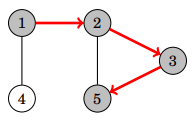
\includegraphics[width=5cm, height=3cm]{graph-example-traverse-2.png}
 \caption{step 2: Sample Graph After Traversing}
    \label{fig:graph-example-traverse-2}
\end{figure}

The neighbors of node 5 are 2 and 3, but the search has already visited both of them, so it is time to return to the previous nodes. Also the neighbors of nodes 3 and 2 have been visited, so we next move from node 1 to node 4:

\begin{figure}[h]
    \centering
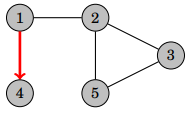
\includegraphics[width=5cm, height=3cm]{graph-example-traverse-3.png}
 \caption{step 3: Sample Graph After Traversing}
    \label{fig:graph-example-traverse-3}
\end{figure}

After this, the search terminates because it has visited all nodes.
The time complexity of depth-first search is O(n+ m) where n is the number of nodes and m is the number of edges, because the algorithm processes each node and edge once.
\newpage

\subsubsection{Implementation}

Depth-first search can be conveniently implemented using recursion. The following function dfs begins a depth-first search at a given node. The function assumes that the graph is stored as adjacency lists in an array, so the following representation is array of vectors: 
\begin{lstlisting}{c++}
        vector<int> adj[N]; //vector< vector<int> > adj; //int adj[N][N];
\end{lstlisting}

Also, we will maintain a visited array to avoid cycles:
\begin{lstlisting}{c++}
        bool visited[N]; //To not visit node more than one time
\end{lstlisting}

The following function will keep get source node, or the start node to start traversing via the graph nodes, such that the visited array keeps track of the visited nodes. Initially, each array value is false, and
when the search arrives at node s, the value of visited[s] becomes true. The function can be implemented as follows:
\begin{lstlisting}{c++}
        typedef vector<int> vi; //vi is abbreviation for vector<int>
        bool visited; //global variable, initially all values are set to false
        void dfs(int s) { // DFS for normal usage: as graph traversal algorithm
                visited[s] = true;// important: we mark this vertex as visited
                for (int j = 0; j < (int)AdjList[s].size(); j++) { // default DS: AdjList
                int child = AdjList[s][j]; //child is a (neighbor) for his parent -parent is the node current node in upper bound level-
                if (visited[child] == false) //important check to avoid cycle
                    dfs(chlid); //recursively visits unvisited neighbors of vertex chlid, and child will be a parent for its neighboors
        } }
\end{lstlisting}
It is the same as the previous functon, but changing just two lines to of this code to be fammiliar more and more with the code:
\begin{lstlisting}{c++}
        typedef vector<int> vi; //vi is abbreviation for vector<int>
        vector<bool> visited; //global variable, initially all values are set to false
        void dfs(int s) { // DFS for normal usage: as graph traversal algorithm
                if (visited[s]) return;//important check to avoid cycle
                visited[s] = true;//important: we mark this vertex as visited
                for (int j = 0; j < (int)AdjList[s].size(); j++) { // default DS: AdjList
                int child = AdjList[s][j]; //child is a (neighbor) for his parent -parent is the node current node in upper bound level-
                    dfs(chlid); //recursively visits unvisited neighbors of vertex chlid, and child will be a parent for its neighboors
        } }
\end{lstlisting}




But for an awesome small words of codes. We can get some help from benefits of c++14, to change the syntax to be a bit samller than before:
\begin{lstlisting}{c++}
        void dfs(int s) {
                if (visited[s]) return; //important check to avoid cycle and if the current node was visited BACKTRACK 
                visited[s] = true;//important: we mark this vertex as visited
                // process node s
                for (auto child: adj[s]) {
                       dfs(child);
                }
        }
\end{lstlisting}
\newpage 
But also, it is the same as the previous functon, but changing just two lines to of this code to be fammiliar more and more with the code:
\begin{lstlisting}{c++}
        void dfs(int s) {
                 //if the current node was visited BACKTRACK 
                visited[s] = true//important: we mark this vertex as visited
                // process node s
                for (auto child: adj[s]) {
                    if(!visited[child])//important check to avoid cycle and if the current node was visited BACKTRACK 
                       dfs(child);
                }
        }
\end{lstlisting}

\newpage 

\subsection{Breadth First Search (BFS)}\label{subsec:BFS}
Breadth-first search (BFS) is one of the basic and essential searching algorithms on graphs. BFS visits the nodes in increasing order of their distance from the starting node. Thus, we can calculate the distance from the starting node to all other nodes using breadth-first search. Breadth-first search goes through the nodes one level after another. First the search explores the nodes whose distance from the starting node is 1, then the nodes whose distance is 2, and so on. This process continues until all nodes have been visited.\\
More precisely, the algorithm can be stated as follows: Create a queue q which will contain the vertices to be processed and a Boolean array used[] which indicates for each vertex, if it has been lit (or visited) or not.

Initially, push the source s to the queue and set used[s]=true, and for all other vertices v set used[v]=false. Then, loop until the queue is empty and in each iteration, pop a vertex from the front of the queue. Iterate through all the edges going out of this vertex and if some of these edges go to vertices that are not already lit, set them on fire and place them in the queue.

As a result, when the queue is empty, the "ring of fire" contains all vertices reachable from the source s, with each vertex reached in the shortest possible way. You can also calculate the lengths of the shortest paths (which just requires maintaining an array of path lengths d[]) as well as save information to restore all of these shortest paths (for this, it is necessary to maintain an array of "parents" p[], which stores for each vertex the vertex from which we reached it).   
\subsubsection{Example}
\begin{figure}[h]
    \centering
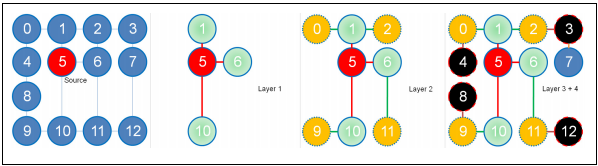
\includegraphics[width=16cm, height=4cm]{BFS-animation.png}
 \caption{Example Animation of BFS.}
    \label{fig:BFS-animation}
\end{figure}

If we run BFS from vertex 5 (i.e. the source vertex s = 5) on the connected undirected
graph shown in Figure 4.3, we will visit the vertices in the following order:

Layer 0: visit 5. Layer 1: visit 1, visit 6, visit 10. Layer 2: visit 0, visit 2, visit 11, visit 9. Layer 3: visit 4, visit 3, visit 12, visit 8. Layer 4: visit 7

\subsubsection{Implementation}
We write code for the described algorithm in C++ to traverse the previous given graph:
\begin{lstlisting}{c++}
        int nodes; //number of nodes
        int source; //source vertex
        
        queue<int> q;
        vector<bool> visited(nodes); //bool used[nodes]; 
        vector< vector<int> > adj;  //adjacency list representation
        //vector<int> adj[n]; as the same as vector< vector<int> > adj;
        q.push(source);
        visited[source] = true; //Source node marked as visited
        while (!q.empty()) {
            int v = q.front();
            q.pop();
            for (int u : adj[v]) {
                if (!used[u]) {
                    visited[u] = true;
                    q.push(u);
                }
            }
            /*
            for (int j = 0; j < adj[v].size(); j++) {
                int child =  adj[v][j];
                if (!visited[child]) {
                    visited[child] = true;
                    q.push(child);
                }
            }
            */
        }
\end{lstlisting}

\newpage

\subsection{Task Assignment Problem (Topological Sort -DAG-)}
Topological sorting of vertices of a Directed Acyclic Graph is an ordering of the vertices $v_1, v_2, ... v_n$ in such a way, that if vertex $u$ comes before vertex $v$ $(u $ → $ v)$ exists in the DAG. 
exists in the DAG. Every DAG has at least one and possibly more topological sort(s). One application of topological sorting is to find a possible sequence of curriculum that a University student has to take to fulfill graduation requirement. Each curricula has certain pre-requisites to be met. These pre-requisites are never cyclic, so they can be modeled as a DAG. Topological sorting this module pre-requisites DAG gives the student a linear list of curriculum be taken one after another without violating the pre-requisites constraints. In order to have a topological sorting the graph must not contain any cycles. In order to prove it, let's assume there is a cycle made of the vertices $v_1, v_2, v_3 ... v_n$. That means there is a directed edge between $v_i$ and $v_{i+1}$ $(1 \le i \lt< n)$ and between $v_n$ and $v_1$. So now, if we do topological sorting then $v_n$ must come before $v_1$ because of the directed edge from $v_n$ to $v_1$. Clearly, $v_{i+1}$ will come after $v_i$, because of the directed from $v_i$ to $v_{i+1}$, that means $v_1$ must come before $v_n$. Well, clearly we've reached a contradiction, here. So topological sorting can be achieved for only directed and acyclic graphs. Like the following figure \ref{fig:topo-sort}
\begin{figure}[h]
    \centering
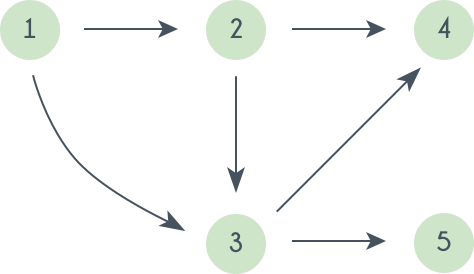
\includegraphics[width=10cm, height=6cm]{topo-sort.png}
 \caption{An Example of Topological Sort (DAG)}\footnotemark
    \label{fig:topo-sort}
\end{figure}
\footnotetext{\url{https://www.hackerearth.com/practice/algorithms/graphs/topological-sort/tutorial/}}

A topological sorting of this graph is: $1$ $2$ $3$ $4$ $5$

There are multiple topological sorting possible for a graph. For the graph given above one another topological sorting is: $1$ $2$ $3$ $5$ $4$

To implement the idea of Topological Sort. There are several algorithms for topological sort. The simplest way is to slightly modify the DFS implementation we presented earlier in subsection \ref{subsection:DFS}.

\newpage

\begin{lstlisting}{c++}
        int nodes;
        stack<int> topsort;
        vector<bool> visited;
        vector< vector<int> > adj;
        void dfs(int node){
        
        	visited[node] = true;
        
        	for(int i = 0; i < adj[node].size(); ++i){
        		int child = adj[node][i];
        		if (!visited[child])	// To avoid cyclic behavior
        			dfs(child);
        	}
        
        	topsort.push(node);// DAG //Possibly, we can use vector to push values in, and reverse it in main function.
        }
\end{lstlisting}

\newpage

\section{Single-Source Shortest Paths}\label{sec:Single-Source Shortest Paths}
\subsection{ Overview and Motivation}
Motivating problem: Given a \textbf{weighted graph} $G$ and a starting source vertex $s$, what are the \textbf{shortest paths} from s to every other vertices of $G$?

\hspace{7mm} This problem is called the \textbf{Single-Source Shortest Paths (SSSP)} problem on a \textbf{weighted graph}. It is a classical problem in graph theory and has many real life applications. For example, we can model the city that we live in as a graph. The vertices are the road junctions. The edges are the roads. The time taken to traverse a road is the weight of the edge. You are currently in one road junction. What is the shortest possible time to reach another certain road junction?

\hspace{7mm}There are efficient algorithms to solve this \textbf{SSSP} problem. If the graph is \textbf{unweighted} (or all edges have equal or constant weight), we can use the efficient \textbf{$O(V + E)$} \textbf{BFS} algorithm shown earlier in subsection \ref{subsec:BFS}. For a general weighted graph, BFS does not work correctly and we should use algorithms like the {$O((V + E) log V )$} \textbf{Dijkstra’s} algorithm or the \textbf{$O(V E)$} \textbf{Bellman Ford’s} algorithm. These various algorithms are discussed below.

\subsection{SSSP on Unweighted Graph}\label{subsec:SSSP on Unweighted Graph}
Let’s revisit subsection \ref{subsec:BFS}. The fact that BFS visits vertices of a graph layer by layer or level by level from a source vertex (see Figure \ref{fig:BFS-animation}).Inan unweighted graph, the distance between two neighboring vertices connected with an edge is simply one unit (constant value).Therefore, the layer count of a vertex that we have seen in subsection \ref{subsec:BFS} is precisely the shortest path length from the source to that vertex. For example in Figure \ref{fig:BFS-animation} the shortest path from vertex 5 to vertex 7, is 4, as 7 is in the fourth layer in BFS sequence of visitation starting from vertex 5.\\
\indent Some programming problems require us to reconstruct (restore - print) the actual shortest path, not just the shortest path length. For example, in Figure \ref{fig:BFS-animation}the shortest path from $5$ to $7$ is $5$ → $1$ → $2$ → $3$ → $7$. This can be easily done using vector of integers $vector<int> parent$. Each vertex $v$ remembers its parent $u$ $(p[v] = u)$.  For this example, vertex $7$ remembers $3$ as its parent, vertex $3$ remembers $2$, vertex $2$ remembers $1$, vertex $1$ remembers $5$ (the source). To reconstruct the actual shortest path, we can do a simple recursion from the last vertex $7$ until we hit the source vertex $5$. The modified BFS code (check the comments) is relatively simple:

\begin{lstlisting}{c++}
        #define INF (int)INT_MAX
        void printPath(int u) { // extract information from              vector<int> p
            if (u == source) { cout << source; return; } // base case, at the source s
            printPath(p[u]); // recursive: to make the output format: s -> ... -> t
            cout << u; 
        }
         int main()
            vector<int> dist(V, INF); dist[source] = 0; // distance from source s to s is 0
            queue<int> q; q.push(source);
            vector<int> p; // addition: the predecessor/parent vector
            while (!q.empty()) {
                int u = q.front(); q.pop();
                for (int j = 0; j < (int)AdjList[u].size(); j++) {
                int child = AdjList[u][j];
                if (dist[child] == INF) {
                        dist[child] = dist[u] + 1;
                        p[child] = u; // addition: the parent of vertex child is u
                        q.push(child);
                    }
                }
            }
            printPath(t), cout << endl; // addition: call printPath from vertex t

\end{lstlisting}

\newpage

\subsection{SSSP on Weighted Graph}\label{subsec:SSSP on Weighted Graph}
If the given graph is weighted, BFS does not work. This is because there can be ‘longer’ path(s) (in terms of number of vertices and edges involved in the path) but has smaller total weight than the ‘shorter’ path found by BFS. For example, in Figure \ref{fig:dijkstra-animation}.

\begin{figure}[h]
    \centering
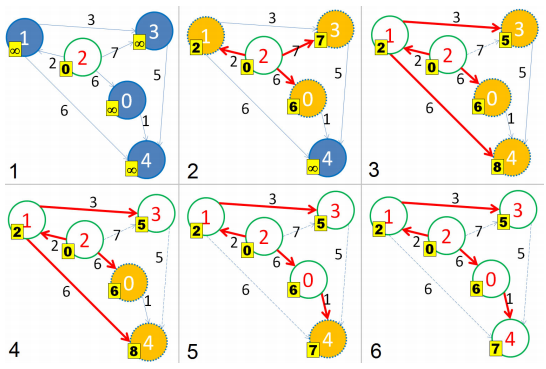
\includegraphics[width=10cm, height=6cm]{dijkstra-animation.png}
 \caption{Dijkstra Animation on a Weighted Graph (from \href{https://vj.z180.cn/52627383937f06635b950dd1efa17b6a?v=1575637256}{\color{red}{UVa 341}})}
    \label{fig:dijkstra-animation}
\end{figure}
\\
\hspace{7mm}The shortest path from source vertex 2 to vertex 3 is not via direct edge 2 → 3 with weight 7 that is normally found by BFS, but a ‘detour’ path: 2 → 1 → 3 with smaller total weight 2 + 3 = 5.

\hspace{7mm}To solve the SSSP problem on weighted graph, we use a greedy Edsger Wybe $Dijkstra’s$ algorithm. There are several ways to implement this classic algorithm. Here we adopt one of the easiest implementation variant that uses built-in C++ STL \lstinline|priority_queue| (or Java \lstinline|PriorityQueue|). This is to keep the length of code minimal—a necessary feature in complexty and programming.

\hspace{7mm}This $Dijkstra’s$ variant maintains a priority queue called $pq$ that stores pairs of vertex
information. The first and the second item of the pair is the distance of the vertex from the
source and the vertex number, respectively. This $pq$ is sorted based on increasing distance
from the source, and if tie, by vertex number.

\hspace{7mm}This \lstinline|pq| only contains one item initially: The base case ($0$, $s$) which is true for the source
vertex. Then, this $Dijkstra’s$ implementation variant repeats the following process until \lstinline|pq|
is empty: It greedily takes out vertex information pair ($d$, $u$) from the front of \lstinline|pq|. If the
distance to $u$ from source recorded in d greater than \lstinline|dist[u]|, it ignores $u$; otherwise, it
process $u$. The reason for this special check is shown below.

\hspace{7mm}When this algorithm process $u$, it tries to relax \footnotemark 
\footnotetext{The operation: relax(u, v, weight-u-v) sets dist[v] = min(dist[v], dist[u] + weight-u-v).}
all neighbors $v$ of $u$. Every time it
relaxes an edge $u$ → $v$, it will enqueue a pair (newer/shorter distance to $v$ from source, $v$)
into \lstinline|pq| and leave the inferior pair (older/longer distance to $v$ from source, $v$) inside \lstinline|pq|. This
is called ‘Lazy Deletion’ and it causes more than one copy of the same vertex in \lstinline|pq| with
different distances from source. That is why we have the check earlier to process only the
first dequeued vertex information pair which has the correct/shorter distance (other copies
will have the outdated/longer distance). The code is shown below and it looks very similar
to BFS code shown in subection \ref{subsec:BFS}\newline\newline

\textbf{{\Large{Dijkstra Animation}}}\newline
\begin{figure}[h]
    \centering
\includegraphics[width=10cm, height=6cm]{DijkstraAnimation.gif}
 \caption{Dijkstra Animation on a Weighted Graph (\href{https://upload.wikimedia.org/wikipedia/commons/5/57/Dijkstra_Animation.gif}{\color{blue}{\textbf{Link}}})}
    \label{fig:DijkstraAnimation}
\end{figure}
\\
\newline

\textbf{{\Large{Implementation}}}\newline
\begin{lstlisting}{c++}
        #include<bits/stdc++.h>
        using namespace std;
        
        typedef pair<int, int> ii;
        typedef vector<int> vi;
        typedef vector<ii> vii;
        #define INF INT_MAX
        
        int main() {
          int V, E, s, u, v, w;
          vector<vii> AdjList;
        
          /*
          // Graph in Figure 2.8
          5 7 2
          2 1 2
          2 3 7
          2 0 6
          1 3 3
          1 4 6
          3 4 5
          0 4 1
          */
        
          cin >> V >> E >> s;
        
          AdjList.assign(V, vii()); // assign blank vectors of pair<int, int>s to AdjList
          for (int i = 0; i < E; i++) {
            cin >> u >> v >> w;
            AdjList[u].push_back(ii(v, w));// directed graph
          }
        
          // Dijkstra routine
          vi dist(V, INF); dist[s] = 0; // INF = INT_MAX to avoid overflow
          priority_queue< ii, vector<ii>, greater<ii> > pq; pq.push(ii(0, s)); // (^_|_^) to sort the pairs by increasing distance from s
          while (!pq.empty()) { // main loop
            ii front = pq.top(); pq.pop(); // greedy: pick shortest unvisited vertex
            int d = front.first, u = front.second;
            if (d > dist[u]) continue; // this check is important, see the explanation
            for (int j = 0; j < (int)AdjList[u].size(); j++) {
              ii v = AdjList[u][j]; // all outgoing edges from u
              if (dist[u] + v.second < dist[v.first]) {
                dist[v.first] = dist[u] + v.second;// relax operation
                pq.push(ii(dist[v.first], v.first));
          } } }// note: this variant can cause duplicate items in the priority queue
        
          for (int i = 0; i < V; i++) // index + 1 for final answer
            cout << SSSP( << s << , << i << ) << = << dist[i] << endl;
        
          return 0;
        }
\end{lstlisting}

